%  Titre:      slides.tex
%  Auteur:     Adrien Stalain
%
%  Fait dans le cadre d'un stage à Orange Labs
%

\documentclass[hyperref={pdfpagelabels=false}]{beamer}
\let\Tiny=\tiny
\usepackage[utf8]{inputenc}
\usepackage{lmodern}% http://ctan.org/pkg/lm
\usepackage{minted}
\usepackage{listings}
\usepackage{color}
\usepackage{times}
\usepackage{tikz}
\usepackage{verbatim}
\usepackage[many]{tcolorbox}
\usepackage{hyperref}
\usepackage{stmaryrd}

\hypersetup{
    colorlinks=true,
    linkcolor=white,
    filecolor=magenta,
    urlcolor=cyan,
}

\usetikzlibrary{arrows,shapes}

\usetheme{Warsaw}

\title{Preuve formelle de micro-noyau}
\author{A. Stalain }\institute{Orange Labs - Stagiaire \\[3mm] {\tiny Tuteur - V. Sanchez Leighton}}


\lstdefinelanguage{thy}{
  keywords={definition, primrec,where,lemma,type_synonym},
  keywordstyle=\color{blue}\bfseries,
  keywords=[2]{clarsimp,wp},
  keywordstyle=[2]\color{brown}\bfseries,
  keywords=[3]{apply,done},
  keywordstyle=[3]\color{red}\bfseries,
  identifierstyle=\color{black},
  sensitive=false,
  comment=[s]{(*}{*)},
  commentstyle=\color{purple}\ttfamily,
  escapeinside={@<}{>@},
  literate={∧}{{$\wedge$}}1
           {≠}{{$\neq$}}1
           {≡}{{$\equiv$}}1
           {∃}{{$\exists$}}1
           {∀}{{$\forall$}}1
           {⦃}{{$\{\!|$}}1
           {⦄}{{$|\!\}$}}1
           {⟦}{{$\llbracket$}}1
           {⟧}{{$\rrbracket$}}1
           {⟹}{{$\Longrightarrow$}}1
           {λ}{{$\lambda$}}1
           {´}{{$\acute{}$}}1
           {∉}{{$\notin$}}1
           {é}{{\'e}}1
           {→}{{\tiny$\rightarrow$}}1
           {⇒}{{$\Rightarrow$}}1,
  string=[s]{"}{"},
  stringstyle=\color{black!60}\ttfamily
}
\lstset{
   language=thy,
   extendedchars=true,
   basicstyle=\scriptsize\ttfamily,
   showstringspaces=false,
   showspaces=false,
   tabsize=2,
   breaklines=true,
   showtabs=false
}

\tikzstyle{manual} = [draw, thin, fill=blue!20]
\tikzstyle{manualspec} = [draw, thin, fill=red!20]
\tikzstyle{autom} = [draw, thin, fill=green!20]
\tikzstyle{idea} = [cloud, draw, thin, aspect=2]
\tikzstyle{basicbox} = [draw, thin]

\definecolor{forestgreen}{rgb}{0.13, 0.55, 0.13}

\setbeamercolor{meta}{bg=red!50,fg=black}

\begin{document}

\begin{frame}
\titlepage
\end{frame}

\section{SeL4}

\begin{frame}{SeL4}
  \begin{itemize}
    \item Micro-noyau, de la famille de L4
      \begin{itemize}
        \item Minimaliste
      \end{itemize}
    \item Sécurisé
    \item Performant
    \item Vérifié formellement
  \end{itemize}
\end{frame}

\begin{frame}[fragile]
  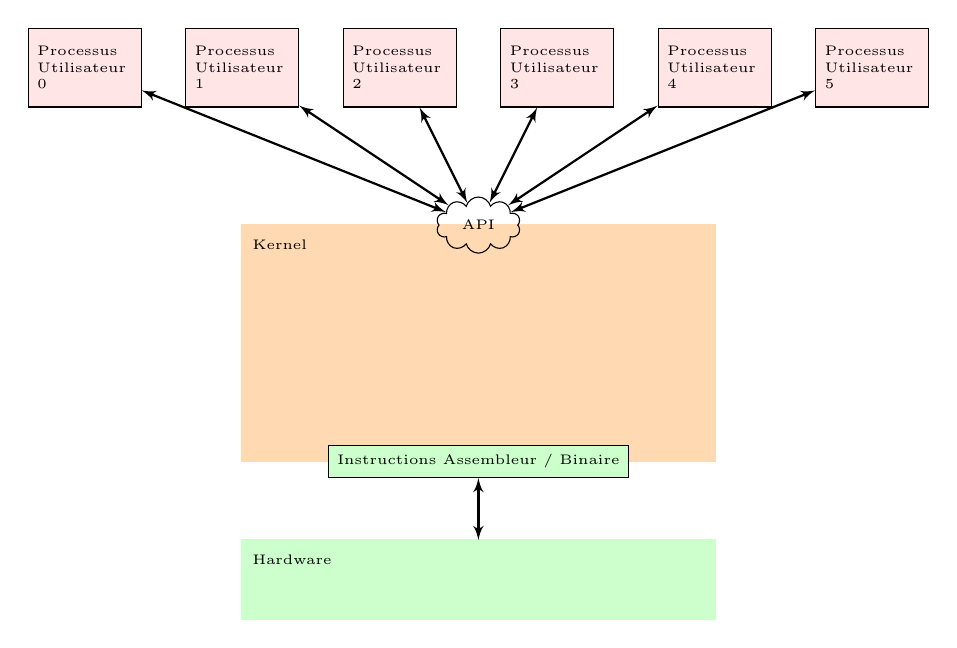
\begin{tikzpicture}[node distance=2cm,auto, >=latex',thick,font=\tiny]

    %kernel
    \draw[fill=orange!30,orange!30] (0, -5) rectangle (6, -8);
    \node[right] at (0,-5.25) {Kernel};
    \node[idea] at (3,-5) (API) {API};
    \node[autom] at (3,-8.) (Bin) {Instructions Assembleur / Binaire};


    %hardware
    \draw[fill=green!20,green!20] (0, -9) rectangle ++(6, -1);
    \node[right] at (0,-9.25) {Hardware};
    \path[<->] (Bin) edge node {} (3,-9);


    %userland processes
     \foreach \x in {0,...,5}
      {
        \node[draw,thin,fill=red!10,minimum size=1cm, text width=1.2cm] at (-2 + 2 * \x,-3) (usr\x) {Processus Utilisateur \x};
        \path[<->] (usr\x) edge node {} (API);
      }

  \end{tikzpicture}
\end{frame}

\begin{frame}<1>[label=proofgraph]{La preuve de SeL4}
\begin{figure}
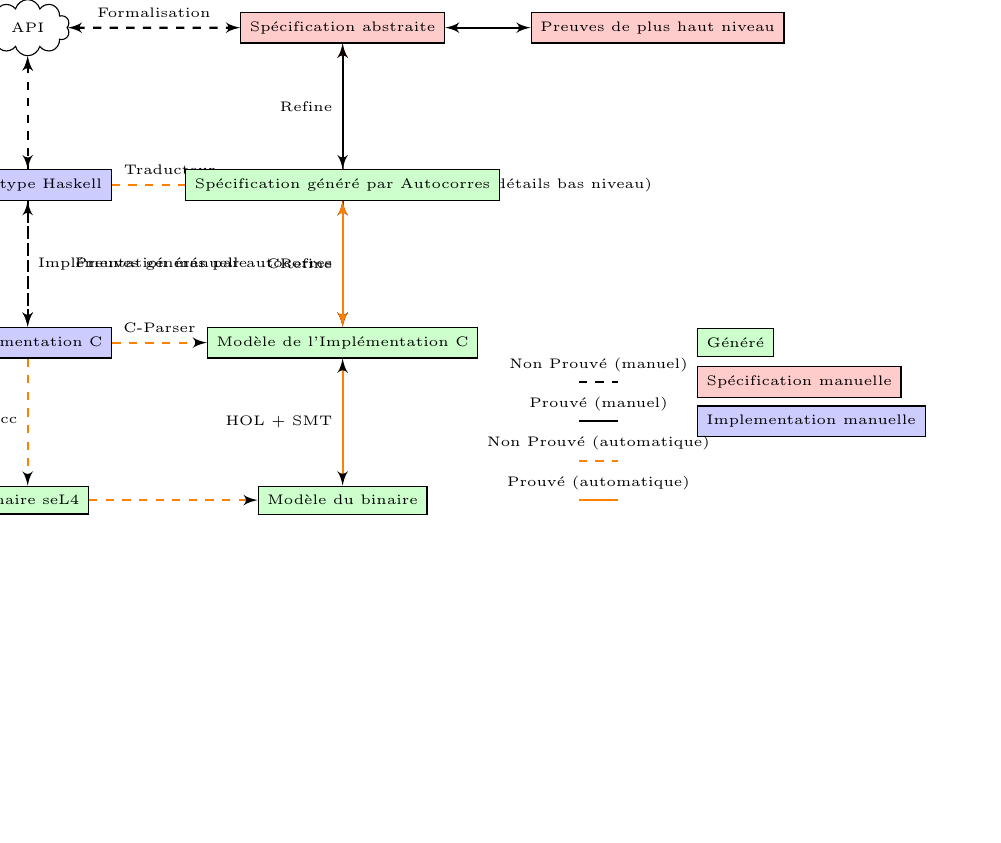
\begin{tikzpicture}[node distance=2cm, auto,>=latex', thick,font=\tiny]
    % We need to set at bounding box first. Otherwise the diagram
    % will change position for each frame.
    \path[use as bounding box] (0,0) rectangle (12,-10);

    \node at (0,-2) (hask) {};

    \path[->]<1-> node[idea, above of=hask] (API) {API}
                  node[manual,below of=hask] (C) {Implémentation C}
                  node[autom, below of=C] (bin) {Binaire seL4};

    \path[->,dashed,draw=orange]<1-> (C) edge node[left] {gcc} (bin);

    \path[<->,dashed]<1-3> (API) edge node[left] {} (C);
    %-
    \path[->]<2-> node[manualspec,right of=API,node distance=4cm] (abspec) {Spécification abstraite};
    \path[<->,dashed]<2-> (API) edge node[above] {Formalisation} (abspec);

    \path[->]<2-> node[autom,right of=C,node distance=4cm] (CMod) {Modèle de l'Implémentation C};
    \path[->,dashed,draw=orange]<2-> (C) edge node[above] {C-Parser} (CMod);

    %-
    \path[<->,draw=red,fill=red]<3> (abspec) edge node [] {Trop compliqué (détails bas niveau)} (CMod);

    %-

    \path[->]<4-7> node[manual,below of=API] (hask2) {Prototype Haskell};
    \path[<->,dashed]<4-7> (hask2) edge node[right] {Implémentation manuelle} (C);
    \path[<->,dashed]<4-7> (API) edge node[left] {} (hask2);

    %-
    \path[->]<4-7> node[autom,right of=hask,node distance=4cm] (ex-spec) {Spécification haut niveau};
    \path[->,dashed,draw=orange]<4-7> (hask2) edge node[above] {Traducteur} (ex-spec);
    %-
    \path[<->,draw]<5-7> (CMod) -- node[left] {CRefine} (ex-spec);
    \path[<->,draw]<5-> (ex-spec) -- node[left] {Refine} (abspec);
    %-

    \path[->]<6-> node[autom, right of=bin,node distance=4cm] (binspec) {Modèle du binaire};

    \path[->,dashed,draw=orange]<6-> (bin) edge node[left] {} (binspec);

    \path[<->,draw=orange]<6-> (binspec) edge node[left] {HOL + SMT} (CMod);
    %-

    \path[<->]<7-> node[manualspec, right of=abspec, node distance=4cm] (highproofs) {Preuves de plus haut niveau}
                  (abspec) edge node {} (highproofs);

    \path[->]<8-> node[autom,right of=hask,node distance=4cm] (autocorres) {Spécification généré par Autocorres};
    \path[<->,draw=orange]<8> (CMod) -- node[left] {Preuves générés par autocorres} (autocorres);

    \draw(8.5,-5) node[manual,right] {Implementation manuelle};
    \draw(8.5,-4) node[autom,right] {Généré};
    \draw(8.5,-4.5) node[manualspec,right] {Spécification manuelle};

    \draw[] (7,-5) -- (7.5,-5) node [midway,above] {Prouvé (manuel)};
    \draw[dashed] (7,-4.5) -- (7.5,-4.5) node [midway,above] {Non Prouvé (manuel)};
    \draw[draw=orange] (7,-6) -- (7.5,-6) node [midway,above] {Prouvé (automatique)};
    \draw[dashed,draw=orange] (7,-5.5) -- (7.5,-5.5) node [midway,above] {Non Prouvé (automatique)};

\end{tikzpicture}
\end{figure}
\end{frame}

\begin{frame}{API}
  \begin{columns}[T] % align columns
    \begin{column}{.15\textwidth}
      
\begin{tikzpicture}[node distance=2cm, auto,>=latex', thick,font=\tiny]
        \path[] node[idea] (API) {API};
      \end{tikzpicture}
    \end{column}%
    \hfill%
    \begin{column}{.83\textwidth}
      La spécification informelle du fonctionnement du système.
      \begin{tcolorbox}[title=Exemple]
        La fonction \texttt{list\_insert\_front} doit insérer un élément en tête de liste chainée.
      \end{tcolorbox}
    \end{column}%
  \end{columns}
\end{frame}

\begin{frame}[fragile]{Implémentation C}
  \begin{columns}[T] % align columns
    \begin{column}{.15\textwidth}
      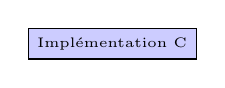
\begin{tikzpicture}[node distance=2cm, auto,>=latex', thick,font=\tiny]
        \path[] node[manual] (C) {Implémentation C};
      \end{tikzpicture}
    \end{column}%
    \hfill%
    \begin{column}{.83\textwidth}
      Le Code source C
      \begin{tcolorbox}[title=Exemple]
        \begin{minted}[fontsize=\tiny]{c}
typedef struct list *list_t;
void list_insert_front(list_t *l, struct list *x)
{
  x->next = *l;
  *l = x;
} 
        \end{minted}
      \end{tcolorbox}
    \end{column}%
  \end{columns}
\end{frame}


\againframe<1>{proofgraph}
\againframe<2>{proofgraph}

\begin{frame}[fragile]{Spécification abstraite}
  \begin{columns}[T] % align columns
    \begin{column}{.15\textwidth}
      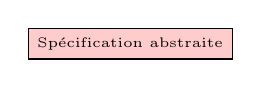
\begin{tikzpicture}[node distance=2cm, auto,>=latex', thick,font=\tiny]
        \path[] node[manualspec] (abspec) {Spécification abstraite};
      \end{tikzpicture}
    \end{column}%
    \hfill%
    \begin{column}{.83\textwidth}
      Une représentation formelle de ce qu'on attends de l'API
      \begin{tcolorbox}[title=Exemple]
        \begin{lstlisting}
lemma list_insert_front_correct : 
  "new ≠ NULL ⟹
    ⦃λs. listp xs l s ∧ is_valid_list_C s new⦄
        list_insert_front l new
    ⦃λ_. listp (new#xs) l⦄!"
        \end{lstlisting}
      \end{tcolorbox}
    \end{column}%
  \end{columns}
\end{frame}

\begin{frame}[fragile]{Modèle de l'implémentation C}
  \begin{columns}[T] % align columns
    \begin{column}{.15\textwidth}
      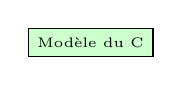
\begin{tikzpicture}[node distance=2cm, auto,>=latex', thick,font=\tiny]
        \path[] node[autom] (CMod) {Modèle du C};
      \end{tikzpicture}
    \end{column}%
    \hfill%
    \begin{column}{.83\textwidth}
      Une représentation formelle du comportement de la fonction.
      \begin{tcolorbox}[title=Exemple]
        \begin{lstlisting}[basicstyle=\tiny]
"all_global_addresses.list_insert_front_body ≡
 TRY
  Guard C_Guard ⦃c_guard ´new⦄
    (Guard C_Guard ⦃c_guard ´l⦄
      (´globals :== t_hrs_'_update (hrs_mem_update (heap_update (Ptr &(´new→[''next_C''])) (h_val (hrs_mem ´t_hrs) ´l)))));;
  Guard C_Guard ⦃c_guard ´l⦄ (´globals :== t_hrs_'_update (hrs_mem_update (heap_update ´l ´new)))
 CATCH SKIP
 END"
        \end{lstlisting}
      \end{tcolorbox}
    \end{column}%
  \end{columns}
\end{frame}

\againframe<3>{proofgraph}
\againframe<4>{proofgraph}

\begin{frame}[fragile]{Prototype Haskell}
  \begin{columns}[T] % align columns
    \begin{column}{.15\textwidth}
      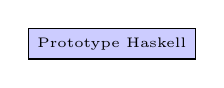
\begin{tikzpicture}[node distance=2cm, auto,>=latex', thick,font=\tiny]
        \path[] node[manual] (hask2) {Prototype Haskell};
      \end{tikzpicture}
    \end{column}%
    \hfill%
    \begin{column}{.83\textwidth}
      \begin{tcolorbox}[title=Exemple]
        \begin{minted}[fontsize=\tiny]{haskell}
insert_front::PPtr ListT -> PPtr List -> Kernel ()
insert_front l new = do
                      mlist <- getListPtr l
                      updateNext new mlist
                      updateListPtr mlist new
        \end{minted}
      \end{tcolorbox}
    \end{column}%
  \end{columns}
\end{frame}

\againframe<4>{proofgraph}
\againframe<5>{proofgraph}
\againframe<6>{proofgraph}
\againframe<7>{proofgraph}

\begin{frame}[fragile]{Autocorres}
  \fbox{%
    \parbox{\textwidth}{%
    \includegraphics[width=\textwidth]{images/autocorres-spec-chain}
    \textbf{\tiny Don't Sweat the Small Stuff, Formal Verification of C Code Without Pain }\\
    \hfill {\tiny -- David Greenaway, Japheth Lim, June Andronick, Gerwin Klein}
    }
    }
    \begin{itemize}
      \item Outil d'abstraction automatique C vers Isabelle
      \item Génère une preuve de correspondance
      \item Développé par le groupe qui développe SeL4
    \end{itemize}
  \begin{columns}[T] % align columns
    \begin{column}{.40\textwidth}
      \begin{minted}[fontsize=\scriptsize]{c}
void list_insert_front
  (list_t *l, struct list *new)
{
  new->next = *l;
  *l = new;
} 
      \end{minted}
    \end{column}
    \begin{column}{.62\textwidth}
      \begin{lstlisting}
"all.list_insert_front' ?l ?new ≡
  do guard(λs. is_valid_list_C s ?new);
   guard(λs. is_valid_list_C'ptr s ?l);
   modify(λs. s[?new→next := s[?l]]);
   modify(λs. s[?l := ?new])
  od"
      \end{lstlisting}
    \end{column}
  \end{columns}

\end{frame}

\againframe<8>{proofgraph}

\section{Preuve}

\begin{frame}[fragile]{Assistant de preuves}
  \begin{columns}[T] % align columns
    \begin{column}{.50\textwidth}
      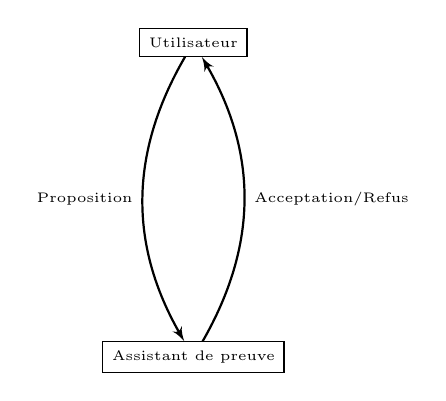
\begin{tikzpicture}[node distance=2cm, auto,>=latex', thick,font=\tiny]
        \path[] node[basicbox] (user) {Utilisateur};
        \path[] node[basicbox,below of=user,node distance=4cm] (pa) {Assistant de preuve};
        \path[->] (user) edge[bend right] node[left] {Proposition} (pa);
        \path[->] (pa) edge[bend right] node[right] {Acceptation/Refus} (user);
      \end{tikzpicture}
    \end{column}%
    \hfill%
    \begin{column}{.50\textwidth}
      \begin{itemize}
        \item Logiciel qui aide l'intéraction entre le noyau du prouveur et l'utilisateur
        \item Permet de résoudre les preuves pas à pas
        \item Isabelle - Coq - Mizar
      \end{itemize}
    \end{column}%
  \end{columns}
\end{frame}

\begin{frame}[fragile]
  \textsc{Triplet de hoare}
  \begin{columns}[T] % align columns
    \begin{column}{.4\textwidth}
      \begin{lstlisting}
"⦃ λs. @<\color{blue}$(x\ mod\ 2) = 0$>@ ⦄
  @<\color{forestgreen}do>@
    @<\color{forestgreen}return (x >> 1)>@
  @<\color{forestgreen}od>@
 ⦃ λr s. @<\color{orange}$r * 2 = x$>@ ⦄"
      \end{lstlisting}
    \end{column}
    \begin{column}{.5\textwidth}
      \begin{minted}[fontsize=\scriptsize]{c}
/* ASSERT : (x % 2) == 0 */
return x >> 1;
/* ASSERT : (ret_value * 2) == x */
      \end{minted}
    \end{column}
  \end{columns}
  Expression vraie quand pour tout état \texttt{s} dans lequel \texttt{\color{blue}précondition} est valide, après l'exécution de \texttt{\color{forestgreen}instructions} dans cet état, alors \texttt{\color{orange}postcondition} sera valide dans le nouvel état.
\end{frame}


\begin{frame}[fragile]{Exemple: liste chainée}
  \begin{minted}[fontsize=\scriptsize]{c}
typedef void *data_ptr;

struct list
{
  struct list *next;
  data_ptr data;
};

typedef struct list *list_t;
  \end{minted}

\end{frame}

\begin{frame}[fragile]{Autocorres avec la syntaxe Lifted heap}
  \begin{tabular}{p{0.5\textwidth} r@{} @{}l}
    \textbf{C} & \multicolumn{2}{c}{\textbf{Isabelle}} \\ \hline
    \begin{minipage}[t]{0.5\textwidth}
      \mint{c}|struct list a;| 
    \end{minipage}
      & $a$ & $\color{gray}{\;:: list\_C} $ \\ \hline

    \begin{minipage}[t]{0.5\textwidth}
      \mint{c}|struct list *a;| 
    \end{minipage}
      & $a$ & $\color{gray}{\;:: list\_C\:ptr}$ \\ \hline

    \begin{minipage}[t]{0.5\textwidth}
      \mint{c}|a.next| 
    \end{minipage}
      & $a{\rightarrow}next$ & $\color{gray}{\;:: list\_C\:ptr}$ \\ \hline

    \begin{minipage}[t]{0.5\textwidth}

    \end{minipage}
      & $s$ & $\color{gray}{\;:: lifted\_globals}$ \\ \hline

    \begin{minipage}[t]{0.5\textwidth}
      \mint{c}|*a| 
    \end{minipage}
      & $s[a]$ & $\color{gray}{\;:: list\_C} $ \\ \hline

    \begin{minipage}[t]{0.5\textwidth}
      \mint{c}|a->next| 
    \end{minipage}
      & $s[a]{\rightarrow}next$ & $\color{gray}{\;:: list\_C ptr}$ \\ \hline


    \begin{minipage}[t]{0.5\textwidth}
      \mint{c}|*a = x| 
    \end{minipage}
      & $s[a := x]$ & $\color{gray}{\;:: lifted\_globals}$ \\
  \end{tabular}

\end{frame}




\begin{frame}[fragile]
  \vfill
  \centering
  \begin{beamercolorbox}[sep=8pt,center,shadow=true,rounded=true]{title}
    \usebeamerfont{title}Preuve de list\_empty\par%
  \end{beamercolorbox}
  \vfill
  \begin{center}
    \begin{minipage}{0.5\textwidth}
      \begin{minted}{c}
void list_empty(list_t *l)
{
  *l = NULL;
}
      \end{minted}
    \end{minipage}
  \end{center}
\end{frame}

\begin{frame}[fragile]{Spécification informelle}
  \textbf{On veut}: Pour \texttt{l} un pointeur (valide) sur pointeur sur node, après l'appel de \texttt{list\_empty l}, \texttt{l} est un pointeur sur liste valide vide. \\
  \begin{center}
    \begin{minipage}{0.5\textwidth}
      \begin{minted}{c}
void list_empty(list_t *l)
{
  *l = NULL;
}
      \end{minted}
    \end{minipage}
  \end{center}
  \vfill
  \only<2->{Une liste valide est une liste dont:}
  \begin{itemize}
    \item<3-> Toutes les nodes sont des zones mémoire valides.
    \item<4-> Soit un pointeur NULL, dans ce cas là, la liste est vide.
    \item<4-> Soit un pointeur sur une node, dans ce cas là, la liste est composée de cette node et de la liste dans le champ \texttt{next} de la node.
  \end{itemize}

\end{frame}

\begin{frame}[fragile]{Définition formelle du concept de liste chainée}
  On définit la fonction \texttt{list}une fonction pour tester l'équivalence entre une liste isabelle et une liste C:
  \vfill
  \begin{onlyenv}<1>
    \begin{lstlisting}
type_synonym node = "list_C ptr"
primrec list :: "node list ⇒ node ⇒ lifted_globals ⇒ bool"  where
    \end{lstlisting}
  \end{onlyenv}
  \begin{onlyenv}<2>
    \begin{lstlisting}
type_synonym node = "list_C ptr"
primrec list :: "node list ⇒ node ⇒ lifted_globals ⇒ bool"  where
list_is_empty:  "list [] p s = (p = NULL)"
    \end{lstlisting}
  \end{onlyenv}
  \begin{onlyenv}<3>
    \begin{lstlisting}
type_synonym node = "list_C ptr"
primrec list :: "node list ⇒ node ⇒ lifted_globals ⇒ bool"  where
list_is_empty:  "list [] p s = (p = NULL)" |
list_is_cons:  "list (x#xs) p s = ( p = x
                              ∧ is_valid_list_C s x
                              ∧ x ≠ NULL
                              ∧ list xs s[x]→next s
                              )"
    \end{lstlisting}
  \end{onlyenv}
\end{frame}

\begin{frame}[fragile]
  On définit \texttt{listp x pt s} comme une expression qui est vraie quand le pointeur sur liste \texttt{struct list **pt} contient exactement les nodes de \texttt{x} dans l'état global \texttt{s}.
  \vfill
  \begin{lstlisting}
definition listp :: "node list ⇒ node ptr ⇒ lifted_globals ⇒ bool" where
  "listp x pt s ≡ (list x s[pt] s
                  ∧ ptr_coerce pt ∉ set x
                  ∧ is_valid_list_C'ptr s pt)"
  \end{lstlisting}
\end{frame}

\begin{frame}[fragile]
  \begin{center}
    \begin{minipage}{0.6\textwidth}
      \begin{onlyenv}<1>
        \begin{lstlisting}
lemma list_empty_correct :
   "⦃ λs. is_valid_list_C'ptr s l ⦄
      all.list_empty' l
    ⦃ λ_. listp [] l ⦄!"
        \end{lstlisting}
  \end{onlyenv}

  \begin{onlyenv}<2>
    \begin{lstlisting}
lemma list_empty_correct :
   "⦃ λs. @<\color{red}is\_valid\_list\_C{\textquotesingle}ptr s l>@ ⦄
      all.list_empty' l
    ⦃ λ_. listp [] l ⦄!"
    \end{lstlisting}
  \end{onlyenv}

  \begin{onlyenv}<3>
    \begin{lstlisting}
lemma list_empty_correct :
   "⦃ λs. is_valid_list_C'ptr s l ⦄
      @<\color{red}all.list\_empty{\textquotesingle} l>@
    ⦃ λ_. listp [] l ⦄!"
    \end{lstlisting}
  \end{onlyenv}

  \begin{onlyenv}<4>
    \begin{lstlisting}
lemma list_empty_correct :
   "⦃ λs. is_valid_list_C'ptr s l ⦄
      all.list_empty' l
    ⦃ λ_. @<\color{red}listp [] l>@ ⦄!"
    \end{lstlisting}
  \end{onlyenv}

  \begin{onlyenv}<5>
    \begin{lstlisting}
lemma list_empty_correct :
   "⦃ λs. is_valid_list_C'ptr s l ⦄
      all.list_empty' l
    ⦃ λ_. listp [] l ⦄@<\color{red}!>@"
    \end{lstlisting}
  \end{onlyenv}
\end{minipage}
  \end{center}

  On prouve que:\\
  \begin{itemize}
    \item<2-> Si \texttt{l} est un \texttt{struct list **} valide.
    \item<3-> Alors, après l'execution de \texttt{list\_empty l}.
    \item<4-> On aura \texttt{l} un pointeur sur liste valide, contenant aucun élément.
    \item<5-> Sans que d'erreur ne se produise, et en un temps fini.
  \end{itemize}

  \vfill
  \hfill
  {\tiny voir (\texttt{proof/Listp.thy})}
\end{frame}

\begin{frame}[fragile]
  \textsc{Traduction par autocorres}
  \begin{tcolorbox}[title=C]
    \begin{minted}{c}
void list_empty(list_t *l)
{
  *l = NULL;
}
    \end{minted}
  \end{tcolorbox}

  \begin{tcolorbox}[title=Isabelle]
    \begin{lstlisting}
"all.list_empty' ?l ≡
  do guard (λs. is_valid_list_C'ptr s ?l);
     modify (λs. s[?l := NULL])
  od"
    \end{lstlisting}
  \end{tcolorbox}
\end{frame}

\begin{frame}

  \begin{beamercolorbox}[sep=8pt,center,shadow=true,rounded=true]{meta}
    \usebeamerfont{title}Démonstration: preuve de \texttt{list\_empty}\par%
  \end{beamercolorbox}
\end{frame}


\begin{frame}[fragile]
  \begin{tabular}{c | c}
    \begin{minipage}[t]{0.4\textwidth}
      \begin{minted}[fontsize=\scriptsize]{c}
void list_empty(list_t *l)
{
  *l = NULL;
}
      \end{minted} 
    \end{minipage}
      &
    \begin{minipage}[t]{0.5\textwidth}
      \begin{minted}[fontsize=\scriptsize]{c}
void list_empty_alt1(list_t *l)
{
  *l = NULL;
  global_variable = (int)l;
}
        \end{minted}
        \vfill
    \end{minipage}
        \\ \hline
        \texttt{list\_empty\_correct} {\color{green}\checkmark} & \texttt{list\_empty\_alt1\_correct} {\color{green}\checkmark} \\
        \texttt{list\_empty\_pure} {\color{green}\checkmark} & \texttt{list\_empty\_alt1\_pure} {\color{red}\texttimes}

  \end{tabular}
  \vfill
        {\tiny \hfill Preuves trouvables dans \texttt{proof/Listp.thy}}
\end{frame}

%%%%%%%%%%%%%%%%%%
% LIST SINGLETON %
%%%%%%%%%%%%%%%%%%

\begin{frame}[fragile]
  \vfill
  \centering
  \begin{beamercolorbox}[sep=8pt,center,shadow=true,rounded=true]{title}
    \usebeamerfont{title}Preuve de list\_singleton\par%
  \end{beamercolorbox}
  \vfill
  \begin{center}
    \begin{minipage}{0.8\textwidth}
      \begin{minted}[fontsize=\scriptsize]{c}
void list_singleton(list_t *l, struct list *x)
{
  *l = x;
}
      \end{minted}
    \end{minipage}
  \end{center}
\end{frame}

\begin{frame}[fragile]{Spécification informelle}
  \textbf{On veut}: Pour \texttt{l} un pointeur sur une liste valide, après l'appel de la fonction \texttt{list\_singleton l x}, l pointera sur une liste avec comme seul elément \texttt{x}. \\
  \vfill
  \begin{center}
    \begin{minipage}{0.8\textwidth}
      \begin{minted}[fontsize=\scriptsize]{c}
void list_singleton(list_t *l, struct list *x)
{
  *l = x;
}
      \end{minted}
    \end{minipage}
  \end{center}

\end{frame}

\begin{frame}[fragile]{Spécification formelle}
  \begin{center}
    \begin{minipage}{0.85\textwidth}
      \begin{onlyenv}<1>
        \begin{lstlisting}
lemma list_singleton_correct :
 "⟦ x ≠ NULL ; x ≠ ptr_coerce l ⟧ ⟹ 
  ⦃λs. is_valid_list_C s x ∧ is_valid_list_C'ptr s l⦄
    all.list_singleton' l x
  ⦃λ _. listp [x] l ⦄!"
        \end{lstlisting}
      \end{onlyenv}

    \begin{onlyenv}<2>
    \begin{lstlisting}
lemma list_singleton_correct :
 "⟦ @<\color{red}x $\neq$ NULL>@ ; @<\color{red}x $\neq$ ptr\_coerce l>@ ⟧ ⟹ 
  ⦃λs. is_valid_list_C s x ∧ is_valid_list_C'ptr s l⦄
    all.list_singleton' l x
  ⦃λ _. listp [x] l ⦄!"
    \end{lstlisting}
  \end{onlyenv}

  \begin{onlyenv}<3>
    \begin{lstlisting}
lemma list_singleton_correct :
 "⟦ x ≠ NULL ; x ≠ ptr_coerce l ⟧ ⟹ 
  ⦃λs. @<\color{red}is\_valid\_list\_C s x>@ ∧ @<\color{red}is\_valid\_list\_C{\textquotesingle}ptr s l>@  ⦄
    all.list_singleton' l x
  ⦃λ _. listp [x] l ⦄!"
    \end{lstlisting}
  \end{onlyenv}

  \begin{onlyenv}<4>
    \begin{lstlisting}
lemma list_singleton_correct :
 "⟦ x ≠ NULL ; x ≠ ptr_coerce l ⟧ ⟹ 
  ⦃λs. is_valid_list_C s x ∧ is_valid_list_C'ptr s l⦄
    @<\color{red}all.list\_singleton{\textquotesingle} l x>@
  ⦃λ _. listp [x] l ⦄!"
    \end{lstlisting}
  \end{onlyenv}

  \begin{onlyenv}<5>
    \begin{lstlisting}
lemma list_singleton_correct :
 "⟦ x ≠ NULL ; x ≠ ptr_coerce l ⟧ ⟹ 
  ⦃λs. is_valid_list_C s x ∧ is_valid_list_C'ptr s l⦄
    all.list_singleton' l x
  ⦃λ _. @<\color{red}listp [x] l>@ ⦄!"
    \end{lstlisting}
  \end{onlyenv}
  \begin{onlyenv}<6>
    \begin{lstlisting}
lemma list_singleton_correct :
 "⟦ x ≠ NULL ; x ≠ ptr_coerce l ⟧ ⟹ 
  ⦃λs. is_valid_list_C s x ∧ is_valid_list_C'ptr s l⦄
    all.list_singleton' l x
  ⦃λ _. listp [x] l ⦄@<\color{red}!>@"
    \end{lstlisting}
  \end{onlyenv}
\end{minipage}
  \end{center}

  On prouve que:\\
  \begin{itemize}
    \item<2-> Pour tout \texttt{x} non-nul et \texttt{x $\neq$ (struct list *)l}.
    \item<3-> Si \texttt{l} et \texttt{x} sont des pointeurs valides sur leur types respectifs.
    \item<4-> Alors, après l'execution de \texttt{list\_singleton l x}.
    \item<5-> On aura \texttt{l} un pointeur sur liste valide, contenant uniquement x
    \item<6-> Sans que d'erreurs se produise, et en un temps fini.
  \end{itemize}

  \vfill
  \hfill
  {\tiny voir (\texttt{proof/Listp.thy})}
\end{frame}

\begin{frame}

  \begin{beamercolorbox}[sep=8pt,center,shadow=true,rounded=true]{meta}
    \usebeamerfont{title}Démonstration: preuve de \texttt{list\_singleton}\par%
  \end{beamercolorbox}
\end{frame}

\begin{frame}[fragile]
  \textbf{Problème}: on arrive pas a prouver que:
  \begin{lstlisting}
1. ∀s. [...] ⟹ s[x]→next = NULL
  \end{lstlisting}
  \pause
  \textbf{C'est à dire}:
  \begin{itemize}
    \item Que \texttt{x->next == NULL}.
  \end{itemize}
  \pause
  \textbf{Pourquoi}:
  \begin{itemize}
    \item Si la proposition est fausse, \texttt{x} ne serait pas néssésairement le dernier élément puisque son \texttt{$\rightarrow$next} est pas forcémment \texttt{NULL}.
    \item C'est donc un bug dans la fonction.
  \end{itemize}
  \pause
  \textbf{Solution}:
  \begin{itemize}
    \item Corriger le code source.
  \end{itemize}
\end{frame}

\begin{frame}[fragile]
\textbf{On a donc}:
  \begin{center}
    \begin{minipage}{0.8\textwidth}
      \begin{minted}[fontsize=\scriptsize]{c}
void list_singleton(list_t *l, struct list *x)
{
  *l = x;
  x->next = NULL;
}
      \end{minted}
    \end{minipage}
  \end{center}
  La preuve peut donc permetre de corriger des bugs.
  \vfill
  \hfill
  {\tiny voir (\url{proof/Listp.thy})}
\end{frame}

%%%%%%%%%%%%%%%%%%%%%
% LIST INSERT FRONT %
%%%%%%%%%%%%%%%%%%%%%

\begin{frame}[fragile]
  \vfill
  \centering
  \begin{beamercolorbox}[sep=8pt,center,shadow=true,rounded=true]{title}
    \usebeamerfont{title}Preuve de list\_insert\_front\par%
  \end{beamercolorbox}
  \vfill
  \begin{center}
    \begin{minipage}{0.8\textwidth}
      \begin{minted}[fontsize=\scriptsize]{c}
void list_insert_front(list_t *l, struct list *x)
{
  x->next = *l;
  *l = x;
} 
      \end{minted}
    \end{minipage}
  \end{center}
\end{frame}

\begin{frame}[fragile]{Spécification informelle}
  \textbf{On veut}: Pour \texttt{l} un pointeur sur une liste valide, après l'appel de la fonction \texttt{list\_insert\_front l x}, l pointera sur la même liste mais avec \texttt{x} en tête. \\
  \vfill
  \begin{center}
    \begin{minipage}{0.8\textwidth}
      \begin{minted}[fontsize=\scriptsize]{c}
void list_insert_front(list_t *l, struct list *x)
{
  x->next = *l;
  *l = x;
} 
      \end{minted}
    \end{minipage}
  \end{center}

\end{frame}

\begin{frame}[fragile]{Spécification formelle}
  \begin{center}
    \begin{minipage}{0.8\textwidth}
      \begin{onlyenv}<1>
        \begin{lstlisting}
lemma list_insert_front_correct :
  "x ≠ NULL ⟹
    ⦃λs. listp xs l s ∧ is_valid_list_C s x ⦄
     all.list_insert_front' l x
    ⦃λr. listp (x#xs) l ⦄!"
        \end{lstlisting}
      \end{onlyenv}

    \begin{onlyenv}<2>
    \begin{lstlisting}
lemma list_insert_front_correct :
  "@<\color{red}x $\neq$ NULL>@ ⟹
    ⦃λs. listp xs l s ∧ is_valid_list_C s x ⦄
     all.list_insert_front' l x
    ⦃λr. listp (x#xs) l ⦄!"
    \end{lstlisting}
  \end{onlyenv}

  \begin{onlyenv}<3>
    \begin{lstlisting}
lemma list_insert_front_correct :
  "x ≠ NULL ⟹
    ⦃λs. @<\color{red}listp xs l s $\wedge$ is\_valid\_list\_C s x>@ ⦄
     all.list_insert_front' l x
    ⦃λr. listp (x#xs) l ⦄!"
    \end{lstlisting}
  \end{onlyenv}

  \begin{onlyenv}<4>
    \begin{lstlisting}
lemma list_insert_front_correct :
  "x ≠ NULL ⟹
    ⦃λs. listp xs l s ∧ is_valid_list_C s x ⦄
     @<\color{red}all.list\_insert\_front\textquotesingle l x>@
    ⦃λr. listp (x#xs) l ⦄!"
    \end{lstlisting}
  \end{onlyenv}

  \begin{onlyenv}<5>
    \begin{lstlisting}
lemma list_insert_front_correct :
  "x ≠ NULL ⟹
    ⦃λs. listp xs l s ∧ is_valid_list_C s x ⦄
     all.list_insert_front' l x
    ⦃λr. @<\color{red}listp (x\#xs) l>@ ⦄!"
    \end{lstlisting}
  \end{onlyenv}
  \begin{onlyenv}<6>
    \begin{lstlisting}
lemma list_insert_front_correct :
  "x ≠ NULL ⟹
    ⦃λs. listp xs l s ∧ is_valid_list_C s x ⦄
     all.list_insert_front' l x
    ⦃λr. listp (x#xs) l ⦄@<\color{red}!>@"
    \end{lstlisting}
  \end{onlyenv}
\end{minipage}
  \end{center}

  On prouve que:\\
  \begin{itemize}
    \item<2-> Pour tout \texttt{x} non-nul.
    \item<3-> Si \texttt{l} est un pointeur sur liste valide contenant les éléments \texttt{xs} et \texttt{x} est un \texttt{struct list *} valide.
    \item<4-> Alors, après l'execution de \texttt{list\_insert\_front l x}.
    \item<5-> On aura \texttt{l} un pointeur sur liste valide, contenant x suivi des éléments de xs
    \item<6-> Sans que d'erreurs se produise, et en un temps fini.
  \end{itemize}

  \vfill
  \hfill
  {\tiny voir (\texttt{proof/Listp.thy})}
\end{frame}

\begin{frame}

  \begin{beamercolorbox}[sep=8pt,center,shadow=true,rounded=true]{meta}
    \usebeamerfont{title}Démonstration: preuve de \texttt{list\_insert\_front}\par%
  \end{beamercolorbox}
\end{frame}

\begin{frame}[fragile]
  \textbf{Problème}: on arrive pas a prouver que:
  \begin{lstlisting}
1. ∀s. [...] ⟹ ptr_coerce l ≠ x
2. ∀s. [...] ⟹ x ∉ set xs
  \end{lstlisting}
  \pause
  \textbf{C'est à dire}:
  \begin{itemize}
    \item Que \texttt{(struct list*)l} est différent de \texttt{x}.
    \item Et que \texttt{x} n'est pas déja une node de la liste.
  \end{itemize}
  \pause
  \textbf{Pourquoi}:
  \begin{itemize}
    \item Si la proposition 1 est vraie, on corrompraît la liste.
    \item Si la proposition 2 est vraie, on créérait un cycle dans la liste chainée.
  \end{itemize}
  \pause
  \textbf{Solution}:
  \begin{itemize}
    \item Ajouter ces deux propositions en tant que précondition.
  \end{itemize}
\end{frame}

\begin{frame}[fragile]
\textbf{On a donc}:
  \begin{center}
    \begin{minipage}{0.8\textwidth}
      \begin{lstlisting}
lemma list_insert_front_correct :
  "⟦ x ∉ set xs ; x ≠ NULL ; x ≠ ptr_coerce l ⟧ ⟹
    ⦃λs. listp xs l s ∧ is_valid_list_C s x ⦄
     all.list_insert_front' l x
    ⦃λr. listp (x#xs) l ⦄!"
       \end{lstlisting}
    \end{minipage}
  \end{center}
  La preuve peut donc permetre de corriger des erreurs de spécifications.
  \vfill
  \hfill
  {\tiny voir (\url{proof/Listp.thy})}
\end{frame}


\begin{frame}{Conclusion}
  \begin{itemize}
    \item La preuve formule des garanties (mécaniques) sur des propriétées du programmes.
    \item Ces propriétés sont définies (posés) dans son contexte: La Théorie.
    \item Ce contexte peut être aveugle à certaines choses.
    \item Les projets prouvés ont une valeur que dans ce contexte.
  \end{itemize}
\end{frame}

\begin{frame}[fragile]
  \vfill
  \centering
  \begin{beamercolorbox}[sep=8pt,center,shadow=true,rounded=true]{title}
    \usebeamerfont{title}Questions\par%
  \end{beamercolorbox}
  \begin{center}
  Sources \& Slides disponibles sur \\
    {\small \url{https://github.com/PolyB/isabelle-proof-exemple}}\\
    {\tiny (Pas encore public)}
  \end{center}
\end{frame}

\end{document}
